\documentclass[a4paper]{article}
\usepackage{amsfonts}
\usepackage{amsmath}
\usepackage{amssymb}
\usepackage{graphicx}
\usepackage{extarrows}

\newcommand{\Bgcos}{\operatorname{Bgcos}}

\begin{document}

\noindent \large Auteur: Seda Jusjajeva\\
\noindent \large Studierichting: Informatica\\
\noindent \large Oefeningenreeks 3G nr. 15.4 \\

\medskip

\normalsize


$f(x) = \sin x + \dfrac{1}{2}\sin 2x$ \\

$\operatorname{dom}f = \mathbb{R}$ \\

Nulpunten: $\sin x + \dfrac{1}{2}\sin 2x = 0$ \\

$\Leftrightarrow \sin x + \dfrac{1}{2}(2\sin x\cos x) = 0$ \\

$\Leftrightarrow \sin x + \sin x\cos x = 0$ \\

$\Leftrightarrow\sin x(1+\cos x) = 0$ \\

$\Rightarrow \sin x = 0 \vee \cos x = -1$ \\

$\Rightarrow x = n\pi \wedge x = \pi + 2k\pi$ \\

$\Rightarrow {x \in \mathbb{R}, n \in \mathbb{Z} | x = n\pi}$\\

Periode: $2\pi$ \\

VA: \\

geen VA. \\

HA: \\

Geen HA. \\

SA: \\

geen SA. \\

Tekenonderzoek: \\

$f'(x) = \dfrac{d}{dx}\left(\sin x + \dfrac{1}{2}\sin 2x\right)$ \\

$= \cos x + \dfrac{1}{2}\cdot 2\cos 2x$ \\

$= \cos x + \cos 2x$ \\

$ = 2\cos\left(\dfrac{3x}{2}\right)\cos\left(\dfrac{x}{2}\right)$ \\

$2\cos\left(\dfrac{3x}{2}\right)\cos\left(\dfrac{x}{2}\right) = 0 \Leftrightarrow \cos\left(\dfrac{3x}{2}\right) = 0 \vee \cos\left(\dfrac{x}{2}\right) = 0$ \\

$\Rightarrow x = \dfrac{\pi}{3} + \dfrac{2k\pi}{3} \wedge x = \pi + 2k\pi$ \\

$\Rightarrow {x \in \mathbb{R}, n \in \mathbb{Z} | \dfrac{\pi}{3} + \dfrac{2n\pi}{3}}$ \\

$f''(x) = \dfrac{d}{dx}(\cos x + \cos 2x)$ \\

$= -\sin x - 2\sin 2x$ \\

$ = -\sin x - 4\sin x\cos x$ \\

$= \sin x(-1 - 4\cos x)$ \\

$\sin x(-1 - 4\cos x) = 0 \Leftrightarrow \sin x = 0 \vee \cos x = -\dfrac{1}{4}$ \\

$\Rightarrow x = k\pi \wedge x = \pm \Bgcos\left(-\dfrac{1}{4}\right) + 2k\pi$ \\

$\begin{array}{r|ccccccccccccccc}
    x 	 &          & 0 &      & \dfrac{\pi}{3} &             & \Bgcos\left(-\dfrac{1}{4}\right) &                                     & \pi && 2\pi-\Bgcos\left(-\dfrac{1}{4}\right) && \dfrac{5\pi}{3} && 2\pi& \\ 
    \hline
    f(x)   & -        & 0 & +    & +              & +           & +                                              & -                                   & 0 & - & - & - & - & - & 0 & +\\
    f'(x)  & +        & + & +    & 0              & -           & -                                              & -                                   & 0 & - & - & - & 0 & + & + & +\\
    f''(x) & +        & 0 & -    & -              & -           & 0                                              & +                                   & 0        & - & 0 & + & + & + & 0 & -\\ 
    \hline
    f(x)   & \nearrow & \nearrow & \nearrow       & M(\sqrt{3}) & \searrow                                       & \searrow                            & \searrow & \searrow & \searrow & \searrow & \nearrow & m\left(\dfrac{-3\sqrt{3}}{4}\right) & \nearrow & \nearrow & \nearrow \\
           & \smile   &B(0)      & \frown         & \frown      &                                                & B\left(\dfrac{3\sqrt{15}}{8}\right) &  \smile & B(0) & \frown & \smile & B\left(-\dfrac{3\sqrt{15}}{16}\right)& \smile & \smile& B(0)& \frown
\end{array}$ \\

Grafiek: \\

\begin{figure}[h]
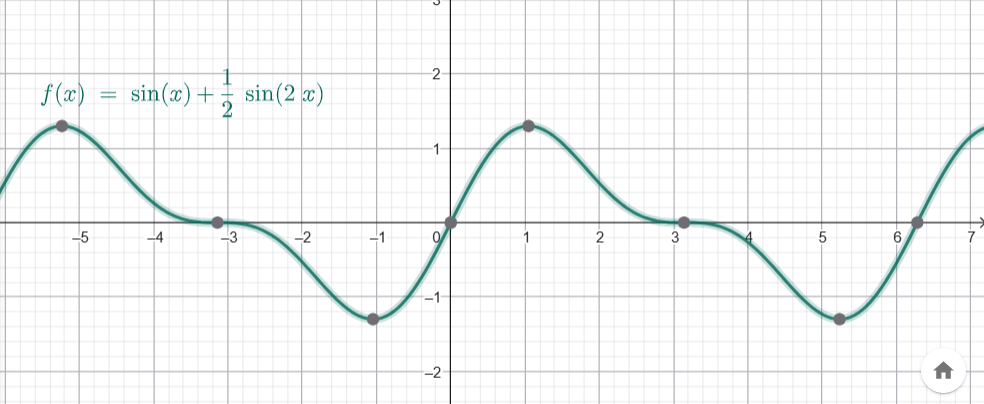
\includegraphics[width=\linewidth]{3G-15.4-seda.jusjajeva.INF.png} \\
\end{figure} 



\begin{thebibliography}{999}
%\bibitem{a} Referentie
\end{thebibliography}
\end{document}